
\documentclass[xcolor=dvipsnames]{beamer}  % for hardcopy add 'trans'

\mode<presentation>
{
  \usetheme{Singapore}
  % or ...
  \setbeamercovered{transparent}
  % or whatever (possibly just delete it)
}

\usefonttheme{professionalfonts}
%\usepackage[english]{babel}
% or whatever
%\usepackage[latin1]{inputenc}
% or whatever
%\usepackage{times}
%\usepackage[T1]{fontenc}
% Or whatever. Note that the encoding and the font should match. If T1
% does not look nice, try deleting the line with the fontenc.

%%%%%%%%%%%%%%%%%%%%%% start my preamble %%%%%%%%%%%%%%%%%%%%%%


\addtobeamertemplate{navigation symbols}{}{%
    \usebeamerfont{footline}%
    \usebeamercolor[fg]{footline}%
    \hspace{1em}%
    \insertframenumber/\inserttotalframenumber
}

\setbeamercolor{footline}{fg=blue}
\setbeamerfont{footline}{series=\bfseries}


%\usepackage{epsfig}
\usepackage{graphicx}
\usepackage{amsmath, amssymb, amsthm}

\usepackage{fancyvrb}

\usepackage{tikz}
\usetikzlibrary{arrows}
\usetikzlibrary{calc}
\usetikzlibrary{intersections}
\usetikzlibrary{decorations}
\usepackage{pgf}
\usepackage{pgfplots}
\pgfplotsset{compat=1.13}

\usepackage{graphviz}
 
\usepackage{verbatim}


\usepackage{algorithmicx,algpseudocode}


%font
\usepackage{mathpazo}
%\usepackage[usenames, dvipsnames]{color}

%\usepackage[linesnumbered, ruled, lined]{algorithm2e}

\usepackage{xr}
\externaldocument[ET-]{et}


\newcommand*{\theorembreak}{\usebeamertemplate{theorem end}\framebreak\usebeamertemplate{theorem begin}}

\newcommand{\newtopic}[1]{\textcolor{Green}{\Large \bf #1}}
\newcommand{\navy}[1]{\textcolor{Blue}{\bf #1}}
\newcommand{\navymth}[1]{\textcolor{Blue}{#1}}
\newcommand{\red}[1]{\textcolor{red}{#1}}


\definecolor{pale}{RGB}{235, 235, 235}
\definecolor{pale2}{RGB}{175,238,238}
\definecolor{turquois4}{RGB}{0,134,139}

% Typesetting code
\definecolor{bg}{rgb}{0.95,0.95,0.95}
\usepackage{minted}
\usemintedstyle{friendly}
\newminted{python}{mathescape,frame=lines,framesep=4mm,bgcolor=bg}
\newminted{ipython}{mathescape,frame=lines,framesep=4mm,bgcolor=bg}
\newminted{julia}{mathescape,frame=lines,framesep=4mm,bgcolor=bg}
\newminted{c}{mathescape,linenos=true}
\newminted{r}{mathescape,  frame=none, baselinestretch=1, framesep=2mm}
\renewcommand{\theFancyVerbLine}{\sffamily
    \textcolor[rgb]{0.5,0.5,1.0}{\scriptsize {\arabic{FancyVerbLine}}}}


\usepackage{stmaryrd}

\newcommand{\Fact}{\textcolor{Brown}{\bf Fact. }}
\newcommand{\Facts}{\textcolor{Brown}{\bf Facts }}
\newcommand{\keya}{\textcolor{turquois4}{\bf Key Idea. }}
\newcommand{\Factnodot}{\textcolor{Brown}{\bf Fact }}
\newcommand{\Eg}{\textcolor{ForestGreen}{Example. }}
\newcommand{\Egs}{\textcolor{ForestGreen}{Examples. }}
\newcommand{\Ex}{{\bf Ex. }}
\newcommand{\Thm}{\textcolor{Brown}{\bf Theorem. }}
\newcommand{\Prf}{\textcolor{turquois4}{\bf Proof.}}
\newcommand{\Ass}{\textcolor{turquois4}{\bf Assumption.}} 
\newcommand{\Lem}{\textcolor{Brown}{\bf Lemma. }}

%source code 



% caligraphic
\usepackage{mathrsfs}
\usepackage{bbm}
\usepackage{subfigure}

\newcommand{\argmax}{\operatornamewithlimits{argmax}}
\newcommand{\argmin}{\operatornamewithlimits{argmin}}

\newcommand\T{{\mathpalette\raiseT\intercal}}
\newcommand\raiseT[2]{\raisebox{0.25ex}{$#1#2$}}

\DeclareMathOperator{\cl}{cl}
%\DeclareMathOperator{\argmax}{argmax}
\DeclareMathOperator{\interior}{int}
\DeclareMathOperator{\Prob}{Prob}
\DeclareMathOperator{\kernel}{ker}
\DeclareMathOperator{\diag}{diag}
\DeclareMathOperator{\sgn}{sgn}
\DeclareMathOperator{\determinant}{det}
\DeclareMathOperator{\trace}{trace}
\DeclareMathOperator{\Span}{span}
\DeclareMathOperator{\rank}{rank}
\DeclareMathOperator{\cov}{cov}
\DeclareMathOperator{\corr}{corr}
\DeclareMathOperator{\range}{rng}
\DeclareMathOperator{\var}{var}
\DeclareMathOperator{\mse}{mse}
\DeclareMathOperator{\se}{se}
\DeclareMathOperator{\row}{row}
\DeclareMathOperator{\col}{col}
\DeclareMathOperator{\dimension}{dim}
\DeclareMathOperator{\fracpart}{frac}
\DeclareMathOperator{\proj}{proj}
\DeclareMathOperator{\colspace}{colspace}

\providecommand{\inner}[1]{\left\langle{#1}\right\rangle}

% mics short cuts and symbols
% mics short cuts and symbols
\newcommand{\st}{\ensuremath{\ \mathrm{s.t.}\ }}
\newcommand{\setntn}[2]{ \{ #1 : #2 \} }
\newcommand{\cf}[1]{ \lstinline|#1| }
\newcommand{\otms}[1]{ \leftidx{^\circ}{#1}}

\newcommand{\fore}{\therefore \quad}
\newcommand{\tod}{\stackrel { d } {\to} }
\newcommand{\tow}{\stackrel { w } {\to} }
\newcommand{\toprob}{\stackrel { p } {\to} }
\newcommand{\toms}{\stackrel { ms } {\to} }
\newcommand{\eqdist}{\stackrel {\textrm{ \scriptsize{d} }} {=} }
\newcommand{\iidsim}{\stackrel {\textrm{ {\sc iid }}} {\sim} }
\newcommand{\1}{\mathbbm 1}
\newcommand{\dee}{\,{\rm d}}
\newcommand{\given}{\, | \,}
\newcommand{\la}{\langle}
\newcommand{\ra}{\rangle}

\renewcommand{\rho}{\varrho}

\newcommand{\htau}{ \hat \tau }
\newcommand{\hgamma}{ \hat \gamma }

\newcommand{\boldx}{ {\mathbf x} }
\newcommand{\boldu}{ {\mathbf u} }
\newcommand{\boldv}{ {\mathbf v} }
\newcommand{\boldw}{ {\mathbf w} }
\newcommand{\boldy}{ {\mathbf y} }
\newcommand{\boldb}{ {\mathbf b} }
\newcommand{\bolda}{ {\mathbf a} }
\newcommand{\boldc}{ {\mathbf c} }
\newcommand{\boldi}{ {\mathbf i} }
\newcommand{\bolde}{ {\mathbf e} }
\newcommand{\boldp}{ {\mathbf p} }
\newcommand{\boldq}{ {\mathbf q} }
\newcommand{\bolds}{ {\mathbf s} }
\newcommand{\boldt}{ {\mathbf t} }
\newcommand{\boldz}{ {\mathbf z} }

\newcommand{\boldzero}{ {\mathbf 0} }
\newcommand{\boldone}{ {\mathbf 1} }

\newcommand{\boldalpha}{ {\boldsymbol \alpha} }
\newcommand{\boldbeta}{ {\boldsymbol \beta} }
\newcommand{\boldgamma}{ {\boldsymbol \gamma} }
\newcommand{\boldtheta}{ {\boldsymbol \theta} }
\newcommand{\boldxi}{ {\boldsymbol \xi} }
\newcommand{\boldtau}{ {\boldsymbol \tau} }
\newcommand{\boldepsilon}{ {\boldsymbol \epsilon} }
\newcommand{\boldmu}{ {\boldsymbol \mu} }
\newcommand{\boldSigma}{ {\boldsymbol \Sigma} }
\newcommand{\boldOmega}{ {\boldsymbol \Omega} }
\newcommand{\boldPhi}{ {\boldsymbol \Phi} }
\newcommand{\boldLambda}{ {\boldsymbol \Lambda} }
\newcommand{\boldphi}{ {\boldsymbol \phi} }

\newcommand{\Sigmax}{ {\boldsymbol \Sigma_{\boldx}}}
\newcommand{\Sigmau}{ {\boldsymbol \Sigma_{\boldu}}}
\newcommand{\Sigmaxinv}{ {\boldsymbol \Sigma_{\boldx}^{-1}}}
\newcommand{\Sigmav}{ {\boldsymbol \Sigma_{\boldv \boldv}}}

\newcommand{\hboldx}{ \hat {\mathbf x} }
\newcommand{\hboldy}{ \hat {\mathbf y} }
\newcommand{\hboldb}{ \hat {\mathbf b} }
\newcommand{\hboldu}{ \hat {\mathbf u} }
\newcommand{\hboldtheta}{ \hat {\boldsymbol \theta} }
\newcommand{\hboldtau}{ \hat {\boldsymbol \tau} }
\newcommand{\hboldmu}{ \hat {\boldsymbol \mu} }
\newcommand{\hboldbeta}{ \hat {\boldsymbol \beta} }
\newcommand{\hboldgamma}{ \hat {\boldsymbol \gamma} }
\newcommand{\hboldSigma}{ \hat {\boldsymbol \Sigma} }

\newcommand{\boldA}{\mathbf A}
\newcommand{\boldB}{\mathbf B}
\newcommand{\boldC}{\mathbf C}
\newcommand{\boldD}{\mathbf D}
\newcommand{\boldI}{\mathbf I}
\newcommand{\boldL}{\mathbf L}
\newcommand{\boldM}{\mathbf M}
\newcommand{\boldP}{\mathbf P}
\newcommand{\boldQ}{\mathbf Q}
\newcommand{\boldR}{\mathbf R}
\newcommand{\boldX}{\mathbf X}
\newcommand{\boldU}{\mathbf U}
\newcommand{\boldV}{\mathbf V}
\newcommand{\boldW}{\mathbf W}
\newcommand{\boldY}{\mathbf Y}
\newcommand{\boldZ}{\mathbf Z}

\newcommand{\bSigmaX}{ {\boldsymbol \Sigma_{\hboldbeta}} }
\newcommand{\hbSigmaX}{ \mathbf{\hat \Sigma_{\hboldbeta}} }

\newcommand{\RR}{\mathbbm R}
\newcommand{\CC}{\mathbbm C}
\newcommand{\NN}{\mathbbm N}
\newcommand{\PP}{\mathbbm P}
\newcommand{\EE}{\mathbbm E \nobreak\hspace{.1em}}
\newcommand{\EEP}{\mathbbm E_P \nobreak\hspace{.1em}}
\newcommand{\ZZ}{\mathbbm Z}
\newcommand{\QQ}{\mathbbm Q}


\newcommand{\XX}{\mathcal X}

\newcommand{\aA}{\mathcal A}
\newcommand{\fF}{\mathscr F}
\newcommand{\bB}{\mathscr B}
\newcommand{\iI}{\mathscr I}
\newcommand{\rR}{\mathscr R}
\newcommand{\dD}{\mathcal D}
\newcommand{\lL}{\mathcal L}
\newcommand{\llL}{\mathcal{H}_{\ell}}
\newcommand{\gG}{\mathcal G}
\newcommand{\hH}{\mathcal H}
\newcommand{\nN}{\textrm{\sc n}}
\newcommand{\lN}{\textrm{\sc ln}}
\newcommand{\pP}{\mathscr P}
\newcommand{\qQ}{\mathscr Q}
\newcommand{\xX}{\mathcal X}

\newcommand{\ddD}{\mathscr D}


\newcommand{\R}{{\texttt R}}
\newcommand{\risk}{\mathcal R}
\newcommand{\Remp}{R_{{\rm emp}}}

\newcommand*\diff{\mathop{}\!\mathrm{d}}
\newcommand{\ess}{ \textrm{{\sc ess}} }
\newcommand{\tss}{ \textrm{{\sc tss}} }
\newcommand{\rss}{ \textrm{{\sc rss}} }
\newcommand{\rssr}{ \textrm{{\sc rssr}} }
\newcommand{\ussr}{ \textrm{{\sc ussr}} }
\newcommand{\zdata}{\mathbf{z}_{\mathcal D}}
\newcommand{\Pdata}{P_{\mathcal D}}
\newcommand{\Pdatatheta}{P^{\mathcal D}_{\theta}}
\newcommand{\Zdata}{Z_{\mathcal D}}




\newcommand{\e}[1]{\mathbbm{E}[{#1}]}
\newcommand{\p}[1]{\mathbbm{P}({#1})}

%\theoremstyle{plain}
%\newtheorem{axiom}{Axiom}[section]
%\newtheorem{theorem}{Theorem}[section]
%\newtheorem{corollary}{Corollary}[section]
%\newtheorem{lemma}{Lemma}[section]
%\newtheorem{proposition}{Proposition}[section]
%
%\theoremstyle{definition}
%\newtheorem{definition}{Definition}[section]
%\newtheorem{example}{Example}[section]
%\newtheorem{remark}{Remark}[section]
%\newtheorem{notation}{Notation}[section]
%\newtheorem{assumption}{Assumption}[section]
%\newtheorem{condition}{Condition}[section]
%\newtheorem{exercise}{Ex.}[section]
%\newtheorem{fact}{Fact}[section]

% Bibliography
\usepackage[authordate,uniquename=false,firstinits,backend=biber,maxcitenames=2]{biblatex-chicago}
\DeclareFieldFormat[article]{title}{#1}
\DeclareFieldFormat[inproceedings]{title}{#1}
\addbibresource{et_newbib.bib}
\renewcommand{\cite}{\textcite}



\setlength{\parskip}{1.5ex plus0.5ex minus0.5ex}


\setlength{\jot}{12pt} 









\title{A Primer in Econometric Theory}

\subtitle
{Lecture 11: Ordinary Least Squares}

\author{John Stachurski \\ \tiny Lectures by Akshay Shanker}





\begin{document}

\begin{frame}
  \titlepage
\end{frame}


\section{Estimation Under OLS}

\begin{frame}\frametitle{Ordinary Least Squares}

    \vspace{2em}
    In chapter~\ref{ET-c:reg} we imposed only mild regularity
    conditions on the data
    
    To provide additional
    interpretation of the estimated coefficients, we now make more
    assumptions --- the classical OLS assumptions
    
    The first assumption is a repetition of assumption~\ref{ET-a:fr} from
    chapter~\ref{ET-c:reg}
    
    \Ass
    \eqref{ET-a:fr2}
    $\boldX$ has full column rank with probability one

\end{frame}

\begin{frame}
    
    \vspace{2em}
    \Ass
    \eqref{ET-a:lols}
    The observations satisfy $\boldy = \boldX \boldbeta + \boldu$ for some 
    unknown $K$-vector of parameters $\boldbeta$ and unobservable vector of
    shocks $\boldu$
    
    \vspace{.7em}
    \Ass
    \eqref{ET-a:bols}
    $\EE [ \boldu \given \boldX ] = \boldzero$
    
    \vspace{.7em}      
    \Ass
    \eqref{ET-a:bols2}
    $\EE [ \boldu \boldu^\T \given \boldX ] = \sigma^2 \boldI$ for some
    unknown $\sigma > 0$
    
    \vspace{.7em}
    Assumption~\ref{ET-a:lols} can be decomposed into the
    separate equations 
    %
    \begin{equation}
        \label{eq:lm}
        y_n = \boldx_n^\T \, \boldbeta + u_n,
        \qquad n = 1, \ldots, N
    \end{equation}

        
\end{frame}

\begin{frame}
    
    \vspace{2em}
    Examples of models that produce relationships in the form of
    \eqref{eq:lm}:
    
    \vspace{.7em}
    \Eg
        \label{eg:cdprod}
        The \navy{Cobb--Douglas production function} relates capital
        and labor inputs with
        output via $y = A k^a \ell^{\delta}$, where $A$ is a random,
        firm-specific productivity term and $a$ and $\delta$ are parameters
        
        Taking logs yields the linear regression model
        %
        \begin{equation*}
            \ln y = \gamma + a \ln k + \delta \ln \ell + u
        \end{equation*}
        %
        where the random term $\ln A$ is represented by $\gamma + u$
\end{frame}

\begin{frame}

    \vspace{2em}
    \Eg
    The \navy{gravity model} relates international trade flows
    between country $\ell$ and country $n$ via the 
    equation $$T_{\ell n} = \lambda \xi_{\ell n} G_\ell^{\alpha} G_n^\beta
    /D_{\ell n}^{\gamma}$$
    
    \begin{itemize}
        \item $T_{\ell n}$ is exports from country
    $\ell$ to country $n$
        \item  $\lambda$ is a constant term
        \item $\xi_{\ell n}$ is a
                shock
        \item $G_\ell$ and $G_n$ are GDP in country 
                $\ell$  and $n$ respectively and $D_{\ell n}$ is 
                distance between them
    \end{itemize}
    
    \vspace{.7em}
    Taking logs gives
    %
    \begin{equation}
        \label{eq:gravity}
        \ln T_{\ell n} 
        = \ln \lambda 
        +  \alpha \ln G_\ell + \beta \ln G_n - \gamma \ln D_{\ell n}
        + \ln \xi_{\ell n}
    \end{equation}
    %

\end{frame}

\begin{frame}
    
    \vspace{2em}
    \Fact\eqref{ET-fa:exfoss}
        If the linearity assumption~\ref{ET-a:lols} holds, then
        %
        \begin{enumerate}
            \item $\boldM \boldy = \boldM \boldu$
            \item $\boldP \boldy = \boldX \boldbeta + \boldP \boldu$
            \item $\rss = \boldu^\T \boldM \boldu$
        \end{enumerate}
        For a proof, see exercise~\ref{ET-ex:exfoss}
    
    \vspace{.7em}
    \Fact\eqref{ET-fa:sruc}
        If assumption~\ref{ET-a:bols} holds, then
        %
        \begin{enumerate}
            \item $\EE [\boldu] = \boldzero$
            \item $\EE [ u_m \given x_{nk} ] = 0$ for any $m, n, k$
            \item $\EE [ u_m x_{nk} ] = 0$ for any $m, n, k$ (orthogonality)
            \item $\cov [ u_m , x_{nk} ] = 0$ for any $m, n, k$
        \end{enumerate}
    %
    For a proof, see exercise~\ref{ET-ex:psruc}
    
\end{frame}

\begin{frame}
    
    \vspace{2em}
    \Fact\eqref{ET-fa:vciu}
        If assumption~\ref{ET-a:bols2} holds, then
        %
        \begin{enumerate}
            \item $\var [\boldu] = \EE [ \boldu \boldu^\T ] = \sigma^2 \boldI$,
            \item $\EE [ u_i^2 \given \boldX ] = \EE [ u_j^2 \given \boldX ] =
                \sigma^2$ for any $i, j$ in $1,\ldots,N$, and 
            \item $\EE [ u_i u_j \given \boldX ] = 0$ whenever $i \not= j$.
        \end{enumerate}
    
    \vspace{.7em}
    Parts 1 and 2 are called \navy{homoskedasticity} and zero correlation
    respectively
    
\end{frame}

\begin{frame}

    \vspace{2em}
    Combining assumptions~\ref{ET-a:bols} and \ref{ET-a:bols2} gives
    %
    \begin{equation*}
        \var [ \boldu  \given \boldX ] 
        := \EE [ \boldu \boldu^\T \given \boldX ]
                -  \EE [ \boldu \given \boldX ] \EE [ \boldu^\T \given \boldX ]
        = \EE [ \boldu \boldu^\T \given \boldX ]
    \end{equation*}
    
    \vspace{.7em}
    Thus the conditional variance--covariance matrix is the diagonal
    matrix $\sigma^2 \boldI$

\end{frame}


\begin{frame}
    
    \vspace{2em}
    The standard estimator of $\boldbeta$ in \eqref{eq:lm} is
    the least squares estimator $\hboldbeta$ defined by Equation \eqref{ET-eq:thelsqe} in ET:
    %
    \begin{equation}
        \label{eq:thelsqe2}
        \hboldbeta := (\boldX^\T \boldX)^{-1} \boldX^\T \boldy
    \end{equation}
    %
    Unlike chapter~\ref{ET-c:reg}, $\hboldbeta$ now understood as an 
    estimator of the unknown parameter vector $\boldbeta$
    
    
    \vspace{.7em}
    Substituting $\boldy = \boldX \boldbeta + \boldu$ into \eqref{eq:thelsqe2} and
    cancelling terms gives the useful comparison
    %
    \begin{equation}
        \label{eq:hg}
        \hboldbeta = 
        \boldbeta + (\boldX^\T \boldX)^{-1} \boldX^\T \boldu 
    \end{equation}
    
\end{frame}

\begin{frame}
    
    \vspace{2em}
    $\hboldbeta$ is also called
    the \navy{OLS estimator} of $\boldbeta$
    
    \vspace{.7em}
    The usual OLS estimator of the parameter $\sigma^2$ introduced in
    assumption~\ref{ET-a:bols2}:
    %
    \begin{equation}
        \label{eq:hatsig}
        \hat \sigma^2 := \frac{\rss}{N - K}
    \end{equation}
    %

\end{frame}

\begin{frame}[fragile]

    \vspace{2em}
    Example that runs the gravity model regression \eqref{eq:gravity} on world
    trade data using Python --- full set of code and data
    can be found at johnstachurski.net/emet

    First import some Python libraries 
    often used for statistics:
    
    \begin{pythoncode}
    import pandas as pd
    import statsmodels.formula.api as smf
    \end{pythoncode}
    
    Rad in the data to a \texttt{pandas DataFrame} from local CSV
    file:
    \small 
    \begin{pythoncode}
    data  = pd.read_csv("./data/gravity_dataset_2013.csv")
    \end{pythoncode}
    
\end{frame}

\begin{frame}[fragile]

    \vspace{2em}
    Build a model using a formula to indicate the regression we want to run
    symbolically (similar to \texttt{R}):
    
    \begin{pythoncode}
    formula = "log(value) ~ log(egdp) \
                + log(igdp) + log(dist)"
    model = smf.ols(formula, data)
    \end{pythoncode}
    
    Perform the estimation and print a table summarizing results:

    \begin{pythoncode}
    result = model.fit(cov_type='HC1')
    print(result.summary())
    \end{pythoncode}

\end{frame}

\begin{frame}[fragile]
%
\small\begin{verbatim}

                   OLS Regression Results                            
===========================================================
Dep. Variable:      log(value)  R-squared:      0.652
Model:                     OLS  Adj. R-squared: 0.652
Method:          Least Squares  F-statistic:    1.203e+04
No. Observations:        19655  Prob (F-statistic): 0.00
Df Residuals:            19651  Log-Likelihood: -47185
Df Model:                    3  AIC:            9.438e+04
Covariance Type:    HC1         BIC:            9.441e+04\documentclass[draft]{article}                                    
==========================================================
                 coef   std err          z         P>|z|   
----------------------------------------------------------
Intercept    -30.2350     0.394    -76.773        0.000   
log(egdp)      1.2783     0.008    153.772        0.000    
log(igdp)      1.0287     0.009    118.885        0.000    
log(dist)     -1.3483     0.023    -58.113        0.000   
=========================================================

\end{verbatim}
%
\end{frame}

\begin{frame}[fragile]

    \vspace{2em}
    Let's check the values for $\hboldbeta$ reported under \texttt{coef}
    coincide with the expression for $\hboldbeta$ given in \eqref{eq:thelsqe2}\
    
    \vspace{.7em}
    First build the design matrix $\boldX$ (see the URL above for details)
    and then compute as follows:
    
    \begin{verbatim}
    betahat = inv(X.T @ X) @ X.T @ y
    \end{verbatim}
    
    The output agrees with the output in the table

    \begin{verbatim}
[-30.23498073   1.27825004   1.02865139  -1.34830012]    
    \end{verbatim}
    
\end{frame}

\begin{frame}[fragile]

    \vspace{2em}
    A \navy{partial
    regression plot} for the linear model just described:
    
    \begin{pythoncode}
import matplotlib.pyplot as plt
import statsmodels.api as sm
fig = plt.figure()
fig = sm.graphics.plot_partregress_grid(result, fig=fig)
    \end{pythoncode}
    
    \begin{itemize}
    \item   horizontal axis --- residuals from regressing 
            \texttt{log(igdp)} on all other
            columns in $\boldX$
    \item   vertical axis --- residuals from regressing the dependent variable
            \texttt{log(value)} on all other
            columns in $\boldX$
    \end{itemize}
    
    \vspace{.7em}
    (Refer to  discussion surrounding equations \eqref{ET-eq:resregy}
    and \eqref{ET-eq:resregx} in ET)
    
\end{frame}

\begin{frame}

    \begin{figure}
    \scalebox{.32}{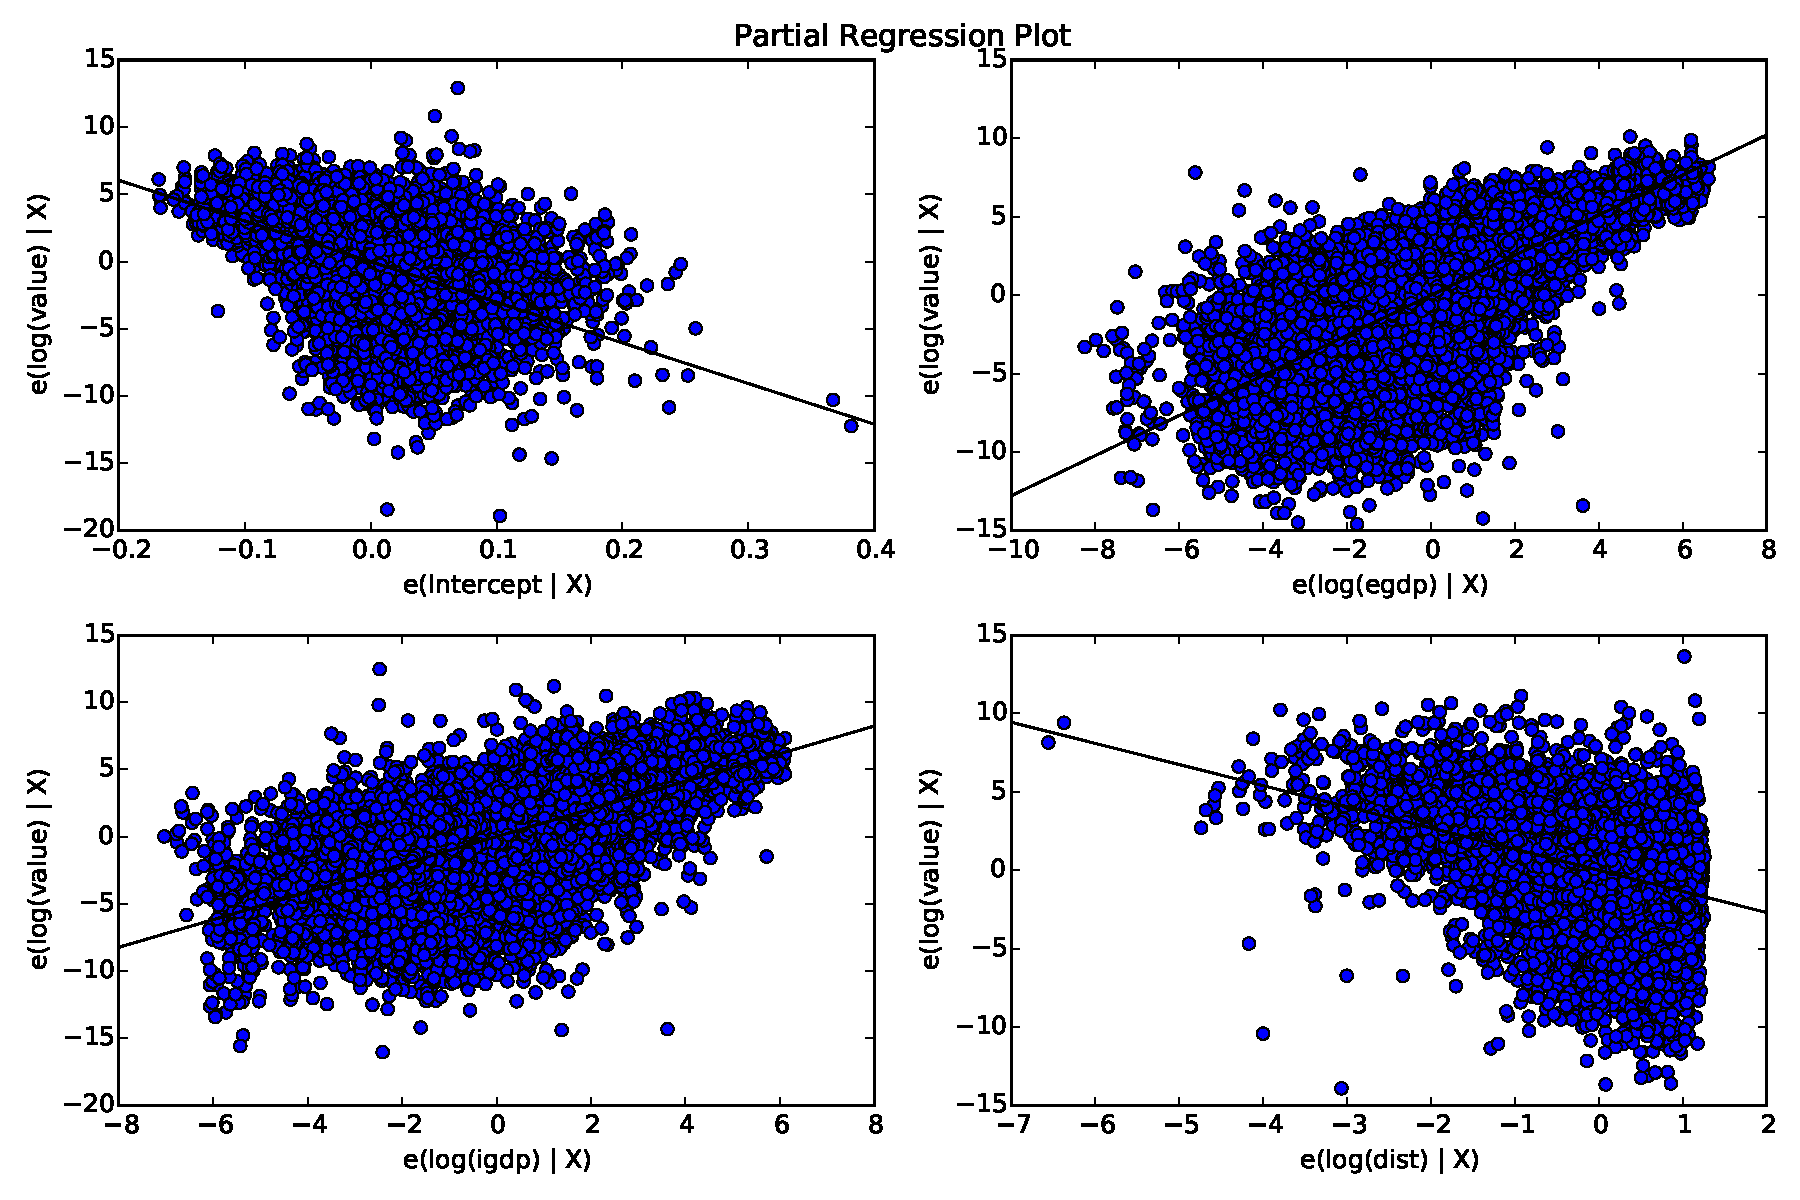
\includegraphics[trim={0em 1em 0em 1em}, clip]{partial_reg_plot.pdf}}
    \caption{\label{f:partial_reg_plot} Partial regression plot for the
    gravity model}
    \end{figure}

\end{frame}

\begin{frame}\frametitle{Finite Sample Properties}

    \vspace{2em}
    \Thm\eqref{ET-t:olsiu}
        If assumptions~\ref{ET-a:fr2}--\ref{ET-a:bols} hold, then 
        %
        \begin{equation}
            \label{eq:hbub}
            \EE \hboldbeta = \EE [\hboldbeta \given \boldX] = \boldbeta
        \end{equation}
        
        If assumption~\ref{ET-a:bols2} also holds, then
        %
        \begin{equation}
            \label{eq:sbub}
          \EE  \hat \sigma^2  = \EE [ \hat \sigma^2 \given \boldX ] = \sigma^2
        \end{equation}
        
\end{frame}

\begin{frame}

    \vspace{2em}
    \Prf
    By (\ref{ET-eq:hg}) and assumption~\ref{ET-a:bols}, we have
        $$\EE [ \hboldbeta \given \boldX ] 
        = \boldbeta 
            + (\boldX^\T \boldX)^{-1} \boldX^\T \EE [ \boldu \given \boldX ] 
        = \boldbeta $$
        
    Taking the unconditional expectation gives \eqref{eq:hbub}

    Regarding \eqref{eq:sbub}, we use the expression for $\rss$ in
    fact~\ref{ET-fa:exfoss}:
    %
    \begin{equation*}
        \EE [\rss \given \boldX]
        = \EE [\boldu^\T \boldM \boldu \given \boldX]
        = \sigma^2 \EE [\boldxi^\T \boldM \boldxi \given \boldX]
        \quad \text{where} \quad
        \boldxi := \sigma^{-1} \boldu
    \end{equation*}
    
\end{frame}

\begin{frame}

    \vspace{2em}
    \Prf (cont.)
    From fact~\ref{ET-fa:eoqf}, $\EE
    [\rss \given \boldX] = \sigma^2 \trace \boldM$
    
    Hence
    %
    \begin{equation*}
        \EE [ \hat \sigma^2 \given \boldX ]
        = \frac{\sigma^2 \trace(\boldM)}{N - K} 
    \end{equation*}
    
    \vspace{.7em}
    By fact~\ref{ET-fa:trop}, we have $\trace \boldM = N - K$
    
    Inserting this into the preceding equation and taking unconditional
    expectations gives \eqref{eq:sbub}  \qedsymbol
    
\end{frame}

\begin{frame}

    \vspace{2em}
    \Thm
    \eqref{ET-t:olsev}
    If assumptions~\ref{ET-a:fr2}--\ref{ET-a:bols2} hold, then
    %
    \begin{equation}
        \label{eq:vhbb}
        \var [\hboldbeta \given \boldX ] = \sigma^2 (\boldX^\T \boldX)^{-1}
    \end{equation}
    %
    For a proof, see exercise~\ref{ET-ex:olsev}
    
    Under the stated conditions, the OLS
    estimator $\hboldbeta$ is best linear unbiased:

    \vspace{.7em}
    \Thm
    \eqref{ET-t:gm} (Gauss-Markov)
        Let assumptions~\ref{ET-a:fr2}--\ref{ET-a:bols2} hold and let $\boldb$ be an
        estimator of $\boldbeta$.  If $\boldb$ is linear and unbiased, then
        %
        \begin{equation*}
             \var [\hboldbeta \given \boldX] \leq \var [\boldb \given \boldX]
        \end{equation*}
        
\end{frame}

\begin{frame}
  
    \vspace{2em}
    Here $\var [\hboldbeta \given \boldX] \leq \var [\boldb \given
    \boldX]$ means  $\var [\boldb \given \boldX] - \var
    [\hboldbeta \given \boldX]$ is nonnegative definite --- one 
    way to assert $\var [\boldb \given \boldX]$ is ``larger''
    
    \begin{itemize}
        \item an implication: $\var [b_k \given \boldX] \geq \var [\hat \beta_k \given \boldX]$ for all $k$
    \end{itemize}
    
    \vspace{.7em}
    Linearity of $\boldb$ means  $\boldb$ is linear as a function of
    $\boldy$, taking $\boldX$ as fixed
    \begin{itemize}
        \item equivalent to requiring 
            $\boldb = \boldC \boldy$ for some matrix $\boldC$; $\boldC$ 
            can depend on $\boldX$ but not $\boldy$
    \end{itemize}
    
    \vspace{.7em}
    Saying $\boldb$ is unbiased means  $\EE [\boldb \given \boldX] = \EE [ \boldC \boldy \given \boldX] =
    \boldbeta$ for all $\boldbeta \in \RR^K$
    
\end{frame}

\begin{frame}

    \vspace{2em}
    \Prf [proof for theorem~\eqref{ET-t:gm}]
    
    Let $\boldb = \boldC \boldy$, as described above, and let $\boldD :=
    \boldC - \boldA$, where $\boldA := (\boldX^\T\boldX)^{-1} \boldX^\T$
    
    \vspace{.7em}
    Then
    %
    \begin{equation}
        \label{eq:bdbb}
        \boldb = \boldC \boldy = \boldD \boldy + \boldA \boldy
        = \boldD (\boldX \boldbeta + \boldu) + \hboldbeta
        = \boldD \boldX \boldbeta + \boldD \boldu + \hboldbeta
    \end{equation}
    
    \vspace{.7em}
    Take conditional expectations and use the fact that $\boldD$ is a
    function of $\boldX$:
    %
    \begin{align*}
        \EE [ \boldb \given \boldX] 
        & = \EE[ \boldD \boldX \boldbeta \given \boldX]  + 
            \EE[ \boldD \boldu \given \boldX ] 
            + \EE[ \hboldbeta \given \boldX] 
            \\
        & = \boldD \boldX \, \EE[ \boldbeta \given \boldX]  + 
             \boldD  \,\EE[\boldu \given \boldX ] 
            + \EE[ \hboldbeta \given \boldX] 
            \\
        & = \boldD \boldX \boldbeta + \boldzero + \boldbeta
    \end{align*}

\end{frame}

\begin{frame}
    
    \vspace{2em}
    Since $\boldb$ is unbiased and, in particular,
    $\EE [ \boldb \given \boldX] = \boldbeta$ for any given $\boldbeta$,
    we have
    %
    \begin{equation*}
        \boldbeta = \boldD \boldX \boldbeta + \boldbeta
        \quad \text{ for all } \boldbeta \in \RR^K
    \end{equation*}
    \begin{equation*}
        \fore
        \boldzero = \boldD \boldX \boldbeta 
        \quad \text{ for all } \boldbeta \in \RR^K
    \end{equation*}
    %
    In light of exercise~\ref{ET-ex:ictz}, we conclude $\boldD \boldX = \boldzero$
    
    \vspace{.7em}
    Combining this result with
    (\ref{eq:bdbb}), we obtain $\boldb = \boldD \boldu + \hboldbeta$

    \vspace{.7em}    
    Hence
    $\boldb$ is equal to the OLS estimator plus zero-mean noise

\end{frame}

\begin{frame}

    To complete the proof, observe
    %
    \begin{multline*}
    \var [ \boldb \given \boldX]
    = \var[ \boldD \boldu + \hboldbeta \given \boldX ]
    \\ = \var[ (\boldD + \boldA ) \boldu \given \boldX ] 
     = (\boldD + \boldA ) \var[ \boldu \given \boldX ] (\boldD + \boldA )^\T
    \end{multline*}
    
    \vspace{.7em}
    Using assumption~\ref{ET-a:bols2} and fact~\ref{ET-fa:owtra}, the right-hand
    side of this expression becomes
    %
    \begin{equation*}
        \sigma^2 (\boldD + \boldA )(\boldD^\T + \boldA^\T)
        = \sigma^2 (\boldD \boldD^\T + \boldD \boldA^\T + \boldA \boldD^\T + \boldA \boldA^\T)
    \end{equation*}
    

\end{frame}

\begin{frame}

    \vspace{2em}
    Since 
    %
    \begin{equation*}
        \boldD \boldA^\T = \boldD \boldX (\boldX^\T \boldX)^{-1} 
        = \boldzero (\boldX^\T \boldX)^{-1}
        = \boldzero 
    \end{equation*}
    %
    and 
    %
    \begin{equation*}
        \boldA \boldA^\T
        =  (\boldX^\T \boldX)^{-1} \boldX^\T \boldX (\boldX^\T \boldX)^{-1} 
        = (\boldX^\T \boldX)^{-1} 
    \end{equation*}
    %
    we conclude
    \begin{equation*}
    \var [ \boldb \given \boldX]
    = \sigma^2 [\boldD \boldD^\T + (\boldX^\T \boldX)^{-1}]
    = \sigma^2 \boldD \boldD^\T + \var [ \hboldbeta \given \boldX]
    \end{equation*}
    %
    The matrix $\sigma^2 \boldD \boldD^\T$ is nonnegative definite, so the proof
    is now done \qedsymbol
    
\end{frame}

\begin{frame}
    \frametitle{Precision of Estimators}

    \vspace{2em}
    By theorem~\ref{ET-t:olsev}, the variance --- covariance matrix of 
    $\hboldbeta$ given $\boldX$ is $\sigma^2 (\boldX^\T \boldX)^{-1}$
    \begin{itemize}
        \item scalar variances of the individual OLS coefficient estimate $\hat
    \beta_1, \ldots, \hat \beta_K$ given by the principal diagonal of this
    matrix
    \end{itemize}
    
    \vspace{.7em}
    Since each $\hat \beta_k$ is unbiased
    (theorem~\ref{ET-t:olsiu}), small variance means
    probability mass concentrated around the true 
    parameter $\beta_k$ --- the estimator has high \navy{precision} 


\end{frame}

\begin{frame}

    \vspace{2em}
    Gauss--Markov Theorem: the OLS estimates will have highest precision
    
    \vspace{.7em}
    Hold the
    estimation technique fixed, as well as the sample size, and vary the
    application
    %
    \begin{itemize}
        \item which problems will have high precision estimates?
        \item which will
            have low precision estimates?
    \end{itemize}
    
    Consider variance of a fixed
    coefficient $\beta_k$ 

\end{frame}

\begin{frame}

    \vspace{2em}
    Write $\boldy = \boldX
    \boldbeta + \boldu$ as
    %
    \begin{equation}
        \label{eq:cfrm}
        \boldy = \boldX_1 \boldbeta_1 + \col_k (\boldX) \beta_k + \boldu
    \end{equation}
    %
    \begin{itemize}
        \item $\col_k(\boldX)$ is the vector of observations of the $k$th regressor
        \item  $\boldX_1$ contains as its columns the observations of the other regressors
        \item $\hboldbeta_1$ is the OLS estimates of the corresponding coefficients
    \end{itemize}
    
\end{frame}

\begin{frame}
    
    \vspace{2em}
    By the FWL theorem:
    %
    \begin{equation}
        \label{eq:exir}
        \hat \beta_k 
        = (\col_k(\boldX)^\T \boldM_1 \col_k(\boldX))^{-1} \col_k(\boldX)^\T \boldM_1 \boldy
    \end{equation}
    %
    \begin{itemize}
        \item $\boldM_1$ is the residual projection 
    $\boldM_1 := \boldI - \boldP_1$
        \item $\boldP_1 := \boldX_1
    (\boldX_1^\T\boldX_1)^{-1} \boldX_1^\T$ projects onto 
    $\colspace \boldX_1$
    \end{itemize}

    \vspace{.7em}
    Apply $\boldM_1$ to both sides of (\ref{eq:cfrm})
    %
    \begin{equation*}
        \boldM_1 \boldy =  \boldM_1 \col_k(\boldX) \beta_k + \boldM_1 \boldu
    \end{equation*}
    %
    Substituting into (\ref{eq:exir}) gives 
    %
    \begin{equation}
        \label{eq:exir2}
        \hat \beta_k 
        = \beta_k + (\col_k(\boldX)^\T \boldM_1 \col_k(\boldX))^{-1}
        \col_k(\boldX)^\T \boldM_1 \boldu
    \end{equation}
    
\end{frame}

\begin{frame}
    
    \vspace{2em}
    Some calculations show (ex.~\ref{ET-ex:voir}) 
    %
    \begin{equation*}
        \label{eq:voir}
        \var[ \hat \beta_k \given \boldX ]
        = \sigma^2 
        (\col_k(\boldX)^\T \boldM_1 \col_k(\boldX))^{-1}
        = \sigma^2 \|\boldM_1 \col_k(\boldX)\|^{-2}
    \end{equation*}
    
    \vspace{.7em}
    Variance of $\hat \beta_k$ depends on:
    \begin{enumerate}
        \item  variance
        $\sigma^2$ of the shock $u$ ---  unavoidable
        \item norm of the vector $\boldM_1
        \col_k \boldX$
    \end{enumerate}
    
\end{frame}

\begin{frame}

    \vspace{2em}
    $\boldM_1 \col_k \boldX$ is the residuals from regressing 
    $\col_k \boldX$ on $\boldX_1$
    
    If $\|\boldM_1 \col_k \boldX\|$ is small, then variance of $\hat \beta_k$ large
    \begin{itemize}
        \item small when $\col_k \boldX$ is
    ``almost'' a linear combination of the other regressors and hence
    close to $\colspace \boldX_1$
    \end{itemize}
    
    \vspace{.7em}
    Then
    %
    \begin{equation*}
        \| \boldM_1 \col_k \boldX \| =
            \| \col_k \boldX  - \boldP_1 \col_k \boldX  \| \approx 0
    \end{equation*}
    %
    Situation referred to as \navy{multicollinearity}
    
\end{frame}


\begin{frame}
 
    \vspace{2em}
    Figure to show  effect of
    multicollinearity on the variance of OLS estimate $\hat \beta_2$
    
    $\boldX$ has two columns related by $\col_2 \boldX = \delta \col_1
    \boldX + (1 - \delta) \boldz$
    
    \begin{itemize}
        \item $\boldz$ is a vector of $N$ independent draws from 
            the standard normal distribution
    \end{itemize}
    
    \vspace{.7em}
    Larger $\delta$ means more
    dependence between $\col_1 \boldX$ and $\col_2 \boldX$
    
    Figure shows the distribution of $\hat \beta_2$ for different values of
    $\delta$
    \begin{itemize}
        \item true parameter is $\beta_2 = 1$
        \item $\hat \beta_2$ is unbiased but its variance increases
    with $\delta$
    \end{itemize}
    
\end{frame}

\begin{frame}

    \begin{figure}
    \centering
    \scalebox{.4}{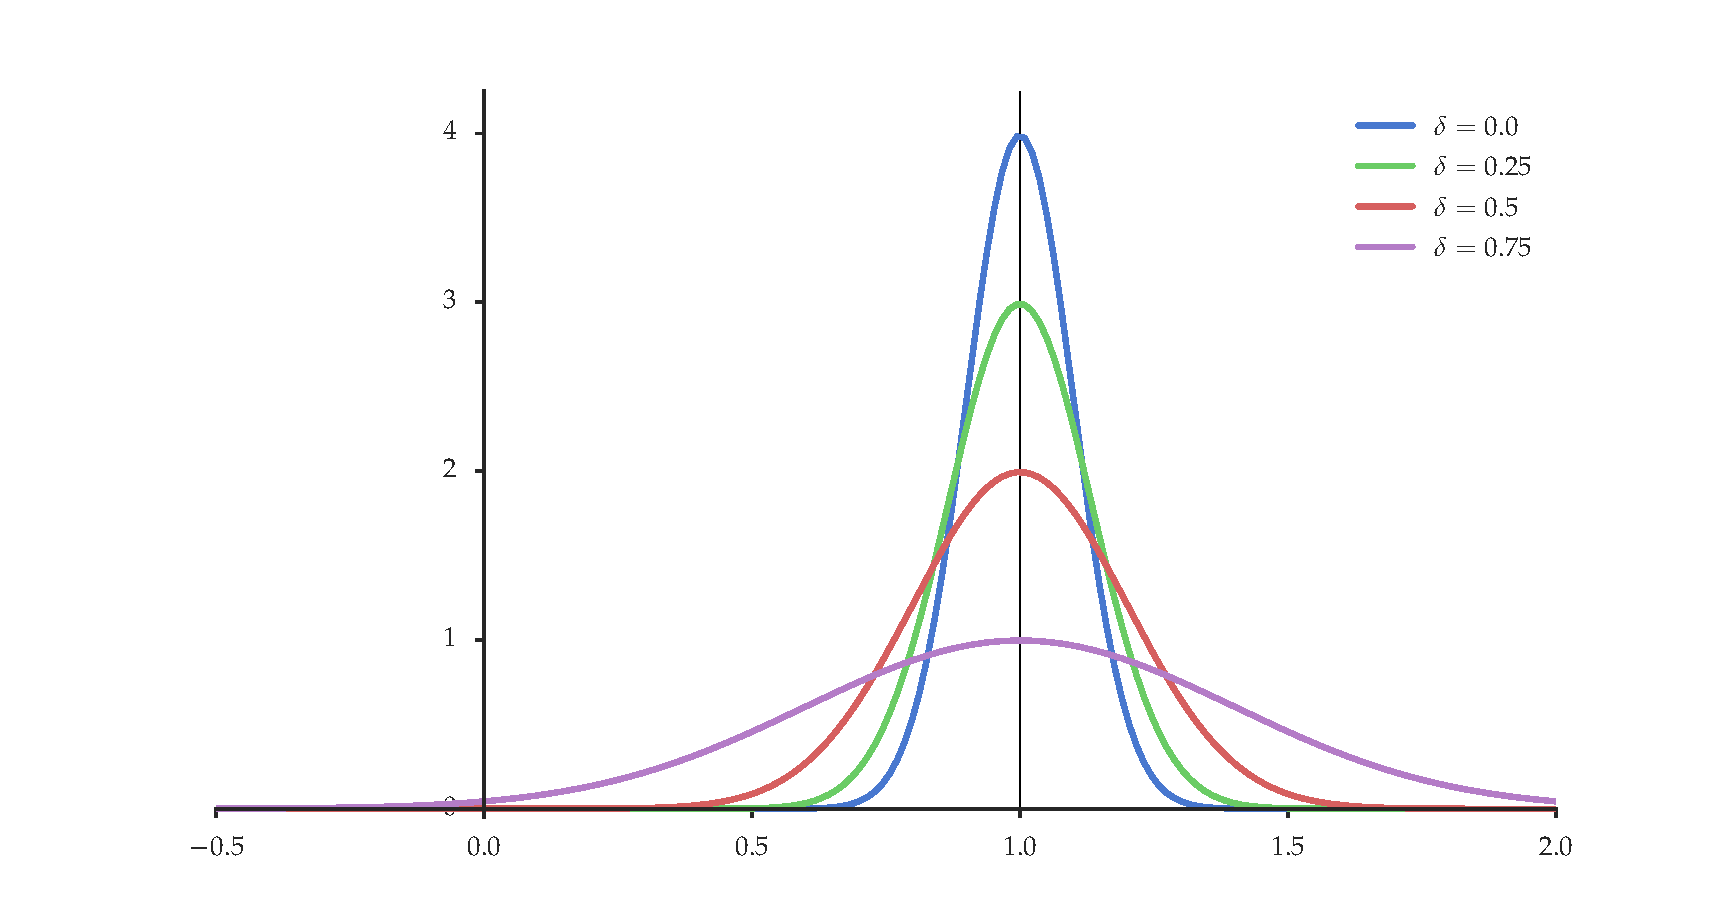
\includegraphics[trim={10em 1em 0em 1em}, clip]{betahat_var.pdf}}
    \caption{\label{f:betahat_var} Distribution of $\hat \beta_2$ when $\col_2 \boldX = \delta \col_1 \boldX + (1 - \delta) \boldz$}
    \end{figure}
    
\end{frame}

\section{Finite Sample Inference}

\begin{frame}
    \frametitle{Inference with Normal Errors}

    \vspace{2em}
    We want to compute confidence intervals or test hypotheses about the
    coefficients in finite samples (i.e., without appealing to asymptotics)
    
    \vspace{.7em}
    \Ass
    \eqref{ET-a:bolsg}
    $\boldX$ and $\boldu$ are independent and $\lL(\boldu) = \nN(\boldzero, \sigma^2 \boldI)$
    
    Assumption~\ref{ET-a:bolsg} implies both assumption~\ref{ET-a:bols} and
    assumption~\ref{ET-a:bols2}
    
\end{frame}

\begin{frame}
    
    \vspace{2em}
    \Thm
    \eqref{ET-t:dools}
    If assumptions~\ref{ET-a:fr2}--\ref{ET-a:lols} and \ref{ET-a:bolsg} hold, then
    %
    \begin{equation*}
        \lL \left[ \, \hboldbeta \given \boldX \, \right] 
        = \nN(\boldbeta, \sigma^2 (\boldX^\T \boldX)^{-1})
    \end{equation*}
    
    \vspace{.7em}
    The theorem implies the distribution of individual coefficient $\hat
    \beta_k$ given $\boldX$ is also normal, with
    %
    \begin{equation}
        \label{eq:dicof}
        \lL \left[ \, \hat \beta_k \given \boldX \, \right] 
        = \lL \left[ \, \bolde_k^\T \, \hboldbeta  \given \boldX \, \right] 
        = \nN(\beta_k, \sigma^2 v_k(\boldX))
    \end{equation}
    %
    Here $v_k (\boldX) :=$ the $(k,k)$th element of $(\boldX^\T \boldX)^{-1}$
    
    (Recall \eqref{ET-eq:mntm} in ET: if $\boldx = (x_1,
    \ldots, x_N)$ is multivariate normal, then 

\end{frame}

\begin{frame}

    \vspace{2em}
    Regarding the distribution of $\hat \sigma^2$, convenient to work with a transformation:
    %
    \begin{equation*}
        \label{eq:Q}
        Q := \frac{\rss}{\sigma^2}
        = (N-K) \frac{\hat \sigma^2}{\sigma^2}
    \end{equation*}
    
    \vspace{.7em}
    \Thm
        \eqref{ET-t:dools2}
        If assumptions~\ref{ET-a:fr2}--\ref{ET-a:lols} and \ref{ET-a:bolsg} hold,
        then
        %
        \begin{equation*}
            \lL \left[ \, Q \given \boldX \, \right] = \chi^2(N - K)
        \end{equation*}
        %
    
    See page~\pageref{ET-t:dools2} in ET for a proof
    
    \Fact
    \eqref{ET-fa:ioes}
    If assumptions~\ref{ET-a:fr2}--\ref{ET-a:lols} and \ref{ET-a:bolsg} hold,
    then the random elements $\hat \sigma^2$ and
    $\hboldbeta$ are independent given $\boldX$ 
    
    See ex.~\ref{ET-ex:ioes}
    
\end{frame}


\begin{frame}\frametitle{The $t$-Test}

    \vspace{2em}
    Consider problem of testing hypothesis about an individual 
    coefficient $\beta_k$
    
    The null hypothesis
    %
    \begin{equation*}
        H_0 \colon \beta_k = \beta_k^0
    \end{equation*}
    %
    where $\beta_k^0$ is any number
    
    \vspace{.7em}
    If $\sigma^2$ is known, construct a
    test of $H_0$ based on:
    %
    \begin{equation}
        \label{eq:istn}
        z_k := \frac{\hat \beta_k - \beta_k} { \sigma \sqrt{v_k(\boldX)} }
        \; \implies \;
        \lL [ \, z_k \given \boldX \, ]
            = \nN(0, 1)
    \end{equation}

\end{frame}

\begin{frame}

    \vspace{2em}
    We don't know $\sigma^2$ ---
    replace $\sigma^2$ with its estimator $\hat \sigma^2$
    
    Some notation:
    %
    \begin{equation*}
        \se(\hat \beta_k) := \sqrt{ \hat \sigma^2 v_k(\boldX)}
    \end{equation*}
    
    \vspace{.7em}
    The term $\se(\hat \beta_k)$ is called the \navy{standard error} of $\hat
    \beta_k$
    
    \vspace{.7em}
    Replace standard deviation
    with its sample estimate $\se(\hat \beta_k)$ and $\beta_k$ with $\beta_k^0$ in
    (\ref{eq:istn}) and obtain the \navy{$t$-statistic}
    %
    \begin{equation*}
        \label{eq:tstat}
        t_k := \frac{\hat \beta_k - \beta_k^0}{\se(\hat \beta_k)}
    \end{equation*}
    
    associated with the hypothesis $H_0$

\end{frame}

\begin{frame}

    \vspace{2em}
    \Thm
    \eqref{ET-t:ttest}
    Let assumptions~\ref{ET-a:fr2}--\ref{ET-a:lols} and \ref{ET-a:bolsg} hold.
    If $H_0$ is true,
    then 
    %
    \begin{equation*}
        \lL \left[ \, t_k \given \boldX \, \right] = 
        \text{Student's t with $N-K$ degrees of freedom}
    \end{equation*}
    
    See page~\pageref{ET-t:ttest} for a proof. 


\end{frame}

\begin{frame}

    \vspace{2em}
    Let $T := |t_k|$ and let a desired size $\alpha$ for our test of $H_0$ be
    given
    
    \vspace{.7em}
    To generate a
    test of size $\alpha$, we choose $c = c_{\alpha}$ to solve $\alpha =
    \PP_{\theta}\{T > c\}$, or
    %
    \begin{equation*}
        1 - \alpha = \PP_{\theta}\{|t_k| \leq c\}
    \end{equation*}
    %
    The solution is
    $c_{\alpha} = F^{-1}(1 - \alpha/2)$
    \begin{itemize}
        \item  $F$ is the Student's $t$ {\sc cdf}
    with $N-K$ degrees of freedom (Equation (\ref{ET-eq:symcdf}) in ET)
    \end{itemize}
    
    \vspace{.7em}
    The
    corresponding $p$-value is $2 F(- |t_k|)$

\end{frame}


\begin{frame}

    \vspace{2em}
    \Eg
    A common implementation of the $t$-test is the
    test that a given coefficient is equal to zero
    
    \vspace{.7em}
    For the $k$th coefficient
    $\beta_k$, this leads to the statistic
    %
    \begin{equation*}
        t_k := \frac{\hat \beta_k}{\se(\hat \beta_k)}
    \end{equation*}
    
    This statistic is sometimes called the \navy{Z-score}
    
    
\end{frame}



\begin{frame}\frametitle{The $F$-Test}

    \vspace{2em}
    Return to the setting of when we discussed the FWL theorem (\S\ref{ET-ss:sap}):
    
    Let $\boldy$ and $\boldX$ be given and let $\hboldbeta$ be the least squares estimator. Let $K_1$ be an integer with $1 \leq
    K_1 < K$, and let
    %
    \begin{itemize}
        \item $\boldX_1$ be a matrix consisting of the first $K_1$ columns of
            $\boldX$,
        \item $\boldX_2$ be a matrix consisting of the remaining $K_2 := K - K_1$
            columns,
        \item $\hboldbeta_1$ be the $K_1 \times 1$ vector consisting of the first
            $K_1$ elements of $\hboldbeta$.
        \item $\hboldbeta_2$ be the $K_2 \times 1$ vector consisting of the
            remaining $K_2$ elements of $\hboldbeta$,
        \item $\boldP_1 := \proj ( \colspace \boldX_1)$, and
        \item $\boldM_1 := \boldI - \boldP_1 =$ the corresponding residual
            projection
    \end{itemize}
    
\end{frame}


\begin{frame}

    \vspace{2em}
    Hypotheses concerning multiple regressors
    
    Null hypothesis:
    %
    \begin{equation*}
        H_0 \colon \boldbeta_2 = \boldzero
    \end{equation*}
    %
    Since
    %
    \begin{equation}
        \label{eq:altr}
        \boldy 
        = \boldX \boldbeta + \boldu 
        = \boldX_1 \boldbeta_1 + \boldX_2 \boldbeta_2 + \boldu
    \end{equation}
    
    \vspace{.7em}
    Under the null hypothesis,
    %
    \begin{equation}
        \label{eq:nullr}
        \boldy = \boldX_1 \boldbeta_1 + \boldu
    \end{equation}

    Let
    %
    \begin{equation*}
        \ussr := \| \boldM \boldy \|^2
        \quad \text{and} \quad
        \rssr := \| \boldM_1 \boldy \|^2
    \end{equation*}
    %
    be the residual sums of squares for the unrestricted regression
    (\ref{eq:altr}) and restricted regression (\ref{eq:nullr})
    
\end{frame}

\begin{frame}

    \vspace{2em}
    Test statistic for our null hypothesis
    %
    \begin{equation}
        \label{eq:fstatr}
        F := \frac{(\rssr - \ussr) / K_2}{ \ussr / (N - K)}
    \end{equation}
    
    \vspace{.7em}
    Large residuals in the restricted regression
    (\ref{eq:nullr}) relative to those in (\ref{eq:altr}) result in large
    values for $F$ --- evidence against the null hypothesis
    
    \vspace{.7em}
    \Thm
    \eqref{ET-t:ftest}
    Let assumptions~\ref{ET-a:fr2}--\ref{ET-a:lols} and \ref{ET-a:bolsg} hold
    
    If $H_0$ is true,
    then, given $\boldX$, the statistic $F$ defined in {\rm
    (\ref{eq:fstatr})} has the $F$ distribution with parameters $(K_2, N - K)$
    
\end{frame}

\begin{frame}

    \vspace{2em}
    \Prf
    
    Let $Q_1 := (\rssr - \ussr)/ \sigma^2$ and let $Q_2 := \ussr/\sigma^2$, so
    that 
    %
    \begin{equation*}
        F = \frac{Q_1 / K_2}{ Q_2 / (N - K)}
    \end{equation*}
    
    \vspace{2em}
    Recall that if $x_1$ and $x_2$ are independent with $\lL(x_i) = \chi^2(k_i)$ for
    $i=1,2$, then 
    %
    \begin{equation*}
        \frac{x_1 / k_1}{x_2 / k_2} 
        \;\;
        \text{ is $F$ distributed with parameters } k_1, k_2
    \end{equation*}
    
\end{frame}


\begin{frame}

    \vspace{2em}
    \Prf (cont.)
    
    Now suffices
    to show that, under the null hypothesis
    %
    \begin{itemize}
        \item[(a)] $Q_1$ is chi-squared with $K_2$ degrees of freedom,
        \item[(b)] $Q_2$ is chi-squared with $N - K$ degrees of freedom, and
        \item[(c)] $Q_1$ and $Q_2$ are independent.
    \end{itemize}
    %
    Part (b) was established in theorem~\ref{ET-t:dools2}
    
    Regarding part (a), under the null hypothesis, 
    %
    \begin{itemize}
        \item $\ussr = \| \boldM \boldy \|^2 = \| \boldM (\boldX_1 \boldbeta_1
            + \boldu) \|^2 = \| \boldM \boldu \|^2 = \boldu^\T \boldM \boldu$ and 
        \item $\rssr = \| \boldM_1 \boldy \|^2 = \| \boldM_1 (\boldX_1 \boldbeta_1 +
            \boldu)\|^2 = \| \boldM_1 \boldu \|^2 = \boldu^\T \boldM_1
            \boldu$.
    \end{itemize}
    
    \vspace{.7em}
    It follows that
    %
    \begin{equation*}
        \rssr - \ussr 
        = \boldu^\T \boldM_1 \boldu  - \boldu^\T \boldM \boldu 
        = \boldu^\T (\boldM_1 - \boldM) \boldu 
    \end{equation*}
    
\end{frame}

\begin{frame}

    \vspace{2em}
    \Prf (cont.)
    
    Using the definitions of $\boldM$ and $\boldM_1$, we obtain
    %
    \begin{multline*}
        Q_1 =
        \frac{\rssr - \ussr}{\sigma^2}
        \\ = \frac{\boldu^\T (\boldI - \boldP_1 - \boldI + \boldP) \boldu}{\sigma^2}
        = (\sigma^{-1} \boldu)^\T (\boldP - \boldP_1) (\sigma^{-1} \boldu)
    \end{multline*}
    
    \vspace{.7em}
    Exercise: show $(\boldP - \boldP_1)$ is symmetric and
    idempotent. Hence
    %
    \begin{multline*}
        \rank(\boldP - \boldP_1)
        = \trace(\boldP - \boldP_1)
       \\ = \trace \boldP - \trace \boldP_1
        = K - K_1 = K_2
    \end{multline*}
    %
   
\end{frame}


\begin{frame}

    \vspace{2em}
    \Prf (cont.)
    Via fact~\ref{ET-fa:mcfi}, we conclude $\lL(Q_1) =\chi^2(K_2)$, as was to be shown
    
    Now we show that, under the null
    hypothesis and taking $\boldX$ as given, $Q_1$ and $Q_2$ are independent
    
    \vspace{.7em}
    $Q_1$ is a function of $(\boldP -
    \boldP_1)\boldu$, while $Q_2$ is a function of $\boldM \boldu$
    
    \begin{itemize}
        \item we show $(\boldP - \boldP_1)\boldu$ and $\boldM \boldu$ are
        independent given $\boldX$ by showing their covariance is zero
    \end{itemize}
    
    Observe
    %
    \begin{multline*}
        \cov [ (\boldP - \boldP_1) \boldu, \boldM \boldu \given \boldX ]
        \\ = \EE [ (\boldP - \boldP_1) \boldu (\boldM \boldu)^\T \given \boldX ]
        = \EE [ (\boldP - \boldP_1) \boldu \boldu^\T \boldM  \given \boldX ]
    \end{multline*}
    
\end{frame}

\begin{frame}

    \vspace{2em}
    \Prf (cont.)
    Since $\boldP$, $\boldP_1$, and $\boldM$ are just functions of $\boldX$,
    the above becomes
    %
    \begin{equation*}
        (\boldP - \boldP_1) \EE [\boldu \boldu^\T\given \boldX ] \boldM  
        = \sigma^2 (\boldP - \boldP_1) \boldM  
        = \sigma^2 (\boldP - \boldP_1) (\boldI - \boldP)
    \end{equation*}
    
    \vspace{.7em}
    Using idempotence and fact~\ref{ET-fa:subsub}, the matrix product on the
    right is
    %
    \begin{equation*}
        (\boldP - \boldP_1) (\boldI - \boldP)
        = \boldP - \boldP^2 - \boldP_1 + \boldP_1 \boldP
        = \boldP - \boldP - \boldP_1 + \boldP_1 
        = \boldzero
    \end{equation*}
    %
    This completes the proof of independence, and hence of
    the theorem  \qedsymbol 
    
\end{frame}

\begin{frame}
    
    \vspace{2em}
    Common F-Test: test that all coefficients 
    of nonconstant regressors are zero
    
    Consider:
    %
    \begin{equation*}
        \boldy = \boldone \beta_1 + \boldX_2 \boldbeta_2  + \boldu
    \end{equation*}
    %
    where $\boldbeta_2$ is the vector of coefficients corresponding to the
    nonconstant regressors. Null hypothesis:
    %
    \begin{equation*}
        \boldy = \boldone \beta_1  + \boldu
    \end{equation*}
    %
    F
    statistic in (\ref{eq:fstatr}) becomes
    %
    \begin{equation*}
        \label{eq:fstat2}
        F = \frac{R^2_c}{1 - R^2_c} \frac{N - K}{K_2}
    \end{equation*}
    %
    (proof is exercise --- see page \pageref{ET-eq:fstat2})
        
    Why is large $F$ is evidence against the
    null?
    
\end{frame}


\section{Problems and Extensions}

\begin{frame}\frametitle{Nonspherical Errors}

    \vspace{2em}
    Heteroskedasticity occurs when the variance of the error term is
    not constant
    across observations
    \begin{itemize}
        \item violate assumption~\ref{ET-a:bols2}
    \end{itemize}
    
    \vspace{.7em}
    Errors \navy{heteroskedastic} if diagonal terms
    of $\EE [ \boldu \boldu^\T \given \boldX ]$ not constant
    
    If the
    off-diagonal terms are nonzero, then the errors are said to have \navy{serial
    correlation}

\end{frame}

\begin{frame}

    \vspace{2em}
    Failure of assumption~\ref{ET-a:bols2} does not alone cause bias in the OLS
    estimator $\hboldbeta$
    
    \vspace{.7em}
    However, without assumption \ref{ET-a:bols2}, no longer true that
    $ \hat \sigma^2$ is unbiased for $\sigma$
    \begin{itemize}
        \item expression $\var [\hboldbeta \given \boldX]
    = \sigma^2 (\boldX^\T \boldX)^{-1}$ from \eqref{eq:vhbb} is no longer valid
        \item Gauss--Markov theorem also breaks down
        \item results on inference we discussed above from \S\ref{ET-ss:ne} no longer valid
    \end{itemize}
    
\end{frame}

\begin{frame}

    \vspace{2em}
    Replace the assumption $\EE [ \boldu \boldu^\T
    \given \boldX ] = \sigma^2 \boldI$ with more general assumption 
    %
    \begin{equation}
        \label{eq:glsa}
        \EE [ \boldu \boldu^\T \given \boldX ] = \boldOmega  
    \end{equation}
    %
    for some positive definite matrix $\boldOmega$
    
    \vspace{.7em}
    Write the variance of the OLS estimator
    $\hboldbeta$ under these conditions as
    %
    \begin{equation*}
        \label{eq:genvar}
        \var [\hboldbeta \given \boldX]
        \\ = \EE [ (\hboldbeta - \boldbeta)(\hboldbeta - \boldbeta)^\T \given \boldX]
        = (\boldX^\T \boldX)^{-1} \boldX^\T \boldOmega  \boldX
            (\boldX^\T \boldX)^{-1}
    \end{equation*}
    
    Maintain assumptions~\ref{ET-a:fr2}--\ref{ET-a:bols}
    
\end{frame}

\begin{frame}

    \vspace{2em}
    Write the variance of the OLS estimator
    $\hboldbeta$ under these conditions as
    %
    \begin{multline*}
        \label{eq:genvar}
        \var [\hboldbeta \given \boldX]
        = \EE [ (\hboldbeta - \boldbeta)(\hboldbeta - \boldbeta)^\T \given \boldX]
        \\ = (\boldX^\T \boldX)^{-1} \boldX^\T \boldOmega  \boldX
            (\boldX^\T \boldX)^{-1}
    \end{multline*}
    
    \vspace{.7em}
    If $\boldOmega$ is known, then we can estimate
    using \navy{generalized least squares}
 
    \begin{itemize}
        \item Cholesky decomposition:
        there exists a nonsingular matrix $\boldC$ such that $\boldC^\T \boldC =
        \boldOmega^{-1}$
        \item  Use $\boldC$ to transform the regression model by multiplying
            both sides of $\boldy = \boldX \boldbeta + \boldu$ by $\boldC$
    \end{itemize}
    
\end{frame}

\begin{frame}
    
    \vspace{2em}
    This gives
    %
    \begin{equation*}
        \boldy_c = \boldX_c \boldbeta + \boldu_c  
        \quad \text{where} \quad
        \boldy_c := \boldC \boldy, \,
        \boldX_c := \boldC \boldX
        \text{ and } \boldu_c := \boldC \boldu
    \end{equation*}
    
    \vspace{.7em}
    Exercise~\ref{ET-ex:gls} asks you to show
    %
    \begin{equation*}
    \label{eq:evug}
    \EE [ \boldu_c \given \boldX_c ] = \boldzero
    \quad \text{and} \quad
    \EE [ \boldu_c \boldu_c^\T \given \boldX_c ] = \boldI
    \end{equation*}
    %
    All OLS assumptions
    satisfied for the transformed data
    
    Use the transformed data to
    estimate $\boldbeta$ via $(\boldX_c^\T \boldX_c)^{-1} \boldX_c^\T \boldy_c$ ---
    recover the best linear unbiased property
    

\end{frame}

\begin{frame}
    
    \vspace{2em}
    The new estimator:
    %
    \begin{equation}
        \label{eq:glsest}
        \hboldbeta_{{\rm GLS}} 
        := (\boldX^\T \boldOmega^{-1} \boldX)^{-1} \boldX^\T \boldOmega^{-1} \boldy
    \end{equation}
    %
    \begin{itemize}
    \item  estimator is the \navy{generalized least squares (GLS) estimator} of
    $\boldbeta$
    \end{itemize}
    
    \vspace{.7em}
    In practice, $\boldOmega$ is rarely known
    
    Estimation difficult unless additional structure is imposed
    \begin{itemize}
        \item $\boldOmega$ is $N \times N$, implying that, absent further
        restrictions, the number of parameters contained in $\boldOmega$ grows 
        \emph{faster} than the sample
    \end{itemize}

\end{frame}

\begin{frame}

    \vspace{2em}
    Assume $\boldOmega$ is diagonal
    \begin{itemize}
        \item rules out correlation but maintains the possibility of heteroskedasticity
    \end{itemize}
    
    One estimator of $\boldOmega$:
    %
    \begin{equation*}
        \hat \boldOmega := \diag(\hat u^2_1, \ldots, \hat u^2_N)
        \quad \text{where} \quad
        \hboldu := \boldM \boldy
    \end{equation*}
    
    Replace $\boldOmega$ with $\hat \boldOmega$ in expression for
    $\var [\hboldbeta \given \boldX]$, get estimate of $\var [\hboldbeta \given \boldX]$:
    %
    \begin{equation*}
        \label{eq:robse}
        \hat \boldV :=
        (\boldX^\T \boldX)^{-1} \boldX^\T \hat \boldOmega  \boldX
            (\boldX^\T \boldX)^{-1}
    \end{equation*}
    %
    Using this in place of the variance estimate $\hat
    \sigma^2 (\boldX^\T \boldX)^{-1}$ to form standard errors, we get
    the \navy{heteroskedasticity-consistent standard errors} proposed by
    \cite{white1980heteroskedasticity}
    
\end{frame}

\begin{frame}\frametitle{Bias}

    \vspace{2em}
    We will look at what happens when  Assumptions~\ref{ET-a:lols}
    and \ref{ET-a:bols} (linearity and exogeneity) fail 
    
    \vspace{.7em}
    Linearity fundamental to OLS. Without lineariry:
    \begin{itemize}
        \item suppose  $y_n =
        f(\boldx_n) + u_n$ for some arbitrary function $f$
        \item  cannot even \emph{ask} if the OLS estimator is unbiased
                because no parameter vector for $\hboldbeta$ to estimate
    \end{itemize}
    
\end{frame}

\begin{frame}\frametitle{Endogeniety Bias} 
    
    \vspace{2em}
    Bias due to
    failure of exogeniety assumption~\ref{ET-a:bols} is called \navy{endogeneity bias}  
    
    \vspace{.7em}
    Recalling Equation \eqref{eq:hg} at the start of the lecture,
    %
    \begin{equation}
        \label{eq:bien}
        \EE [ \hboldbeta \given \boldX ] - 
        \boldbeta = (\boldX^\T \boldX)^{-1} \boldX^\T \EE[ \boldu \given \boldX]
    \end{equation}
    
    Without $\EE [ \boldu \given \boldX ] = \boldzero$, we cannot assert 
    right-hand side is zero, hence $\hboldbeta$ is biased 

\end{frame}

\begin{frame}
    
    \vspace{2em}
    Striving for unbiasedness somewhat misguided. Some degree of bias to
    \begin{itemize}
        \item penalize complexity
        \item recognize empirical distribution not the true
            distribution
    \end{itemize}
    
    \vspace{.7em}
    However, good estimators reduce bias as the sample size increases, so
        that the object they aim to compute can be recovered asymptotically
    \begin{itemize}
        \item not true for the OLS estimator when exogeneity fails
    \end{itemize}
    
\end{frame}

\begin{frame}

    \vspace{2em}
    Recall from theorem~\ref{ET-t:cwa} that:
    $$\hboldbeta \, \toprob  \, \EE[ \boldx \boldx^\T]^{-1} \, \EE[\boldx \, y]$$
    as $N \to \infty$
    
    The right-hand side is the vector of coefficients in the
    best linear predictor
    
    \vspace{.7em}
    If $y = \boldx^\T
    \boldbeta + u$, then
    %
    \begin{equation*}
        \hboldbeta \, 
         \toprob  \,
         \EE[ \boldx \boldx^\T]^{-1} \, \EE[\boldx \, (\boldx^\T \boldbeta + u)]
        =\boldbeta  + \EE[ \boldx \boldx^\T]^{-1} \, \EE[\boldx \,  u]
    \end{equation*}
    %
    With exogeneity we get $\EE[\boldx \,  u] =  \EE[ \boldx \, \EE[ u \given \boldx
    ] ] = 0$ and the OLS estimator is consistent --- cannot
    assert without exogeniety 
 
\end{frame}

\begin{frame}\frametitle{Examples of Exogeniety}

    \vspace{2em}
    Consider again the Cobb--Douglas production function which yields the regression model
    %
    \begin{equation*}
        \ln y_n = \gamma + a \ln k_n + \delta \ln \ell_n + u_n
    \end{equation*}
    %
    \begin{itemize}
        \item $y$ is output, $k$ is capital and $\ell$ is labor
        \item subscript $n$
            indicates observation on the $n$th firmand 
        \item term $u_n$ is a firm specific
        productivity shock
    \end{itemize}
    
    Source of endogeniety bias: firm chooses higher
    levels of capital and labor when it anticipates high productivity in the
    current period
    
\end{frame}

\begin{frame}

    \vspace{2em}
    To illustrate, suppose firm $n$ recieved and observed $u_{n,-1}$ last period
    
    Productivity follows random walk, with $u_n = u_{n, -1} + \eta_n$,
    where $\eta_n$ is zero-mean white noise
    
    \vspace{.7em}
    Firms
    \begin{itemize}
        \item forecast
    period $n$ productivity as $\EE[u_n \given u_{n,-1}] = u_{n,-1}$
        \item  increase labor input when productivity is anticipated
    to be high, with the specific relationship $\ell_n = a + b \EE[u_n \given
    u_{n,-1}]$ for $b > 0$
    \end{itemize}
    
\end{frame}

\begin{frame}

    \vspace{2em}
    With zero-mean shocks:
    %
    \begin{equation*}
        \EE[ \ell_n u_n ] 
        = \EE[ (a + b u_{n,-1})(u_{n,-1} + \eta_n) ]
        = \EE[ b u_{n,-1}^2 ]
    \end{equation*}
    
    \vspace{.7em}
    Strictly positive whenever $u_{n,-1}$ has positive variance
    \begin{itemize}
        \item exogeniety fails as conditions of fact~\ref{ET-fa:sruc} fail
    \end{itemize}

\end{frame}

\begin{frame}
    
    \vspace{2em}
    Now consider data generated according to AR(1) model
    %
    \begin{equation}
        \label{eq:sar1}
        x_0 = 0 
        \quad \text{and} \quad
        x_n = \beta x_{n-1} + u_n
        \quad \text{for } 
        n = 1,\ldots,N
    \end{equation}
    %
    Let $\{u_n\}_{n=1}^N$ be {\sc iid} with distribution $\nN(0,\sigma^2)$
    
    \vspace{.7em}
    The unknown parameters are $\beta$ and $\sigma^2$
    
    Let $\boldy := (x_1,\ldots,x_N)$,
        $\boldx := (x_0,\ldots,x_{N-1})$,
        and $\boldu := (u_1,\ldots,u_N)$,\
        
    Write $N$ equations in (\ref{eq:sar1}) as $\boldy = \beta \boldx +
    \boldu$
    
    The OLS estimate of $\beta$ is
        $\hat \beta := (\boldx^\T \boldx)^{-1} \boldx^\T\boldy$
    
\end{frame}

\begin{frame}

    \vspace{2em}
    If $n \geq m$, then
    we can write $x_n$ as 
    %
    \begin{equation*}
        x_n = \sum_{j=0}^{n-1} \beta^j u_{n-j}
    \end{equation*}
    
    \vspace{.7em}
    Hence $\EE[ x_n u_m] = \sum_{j=0}^{n-1} \beta^j \EE[ u_{n-j} u_m] 
        = \beta^{n - m} \sigma^2$
        
    Once again exogeneity fails since conditions of fact~\ref{ET-fa:sruc} fail
    
\end{frame}

\begin{frame}[fragile]

        \begin{pythoncode}
import numpy as np; import matplotlib.pyplot as plt

N = 25; x = np.zeros(N); beta = 0.9                    
num_reps = 10000; betahat_obs = np.empty(num_reps)
                        
for j in range(num_reps):
    u = np.random.randn(N)
    for t in range(N-1):
        x[t+1] = beta * x[t] + u[t+1]
    y = x[1:]       # x_1 ,..., x_N          
    x_vec = x[:-1]  # x_0, ..., x_{N-1}
    betahat_obs[j]  = np.sum(x_vec * y) \
                        /np.sum(x_vec**2)

plt.hist(betahat_obs, bins=50, alpha=0.6, normed=True)
plt.show()
        \end{pythoncode}

\end{frame}

\begin{frame}
        
    \begin{figure}
       \begin{center}
        \scalebox{.4}{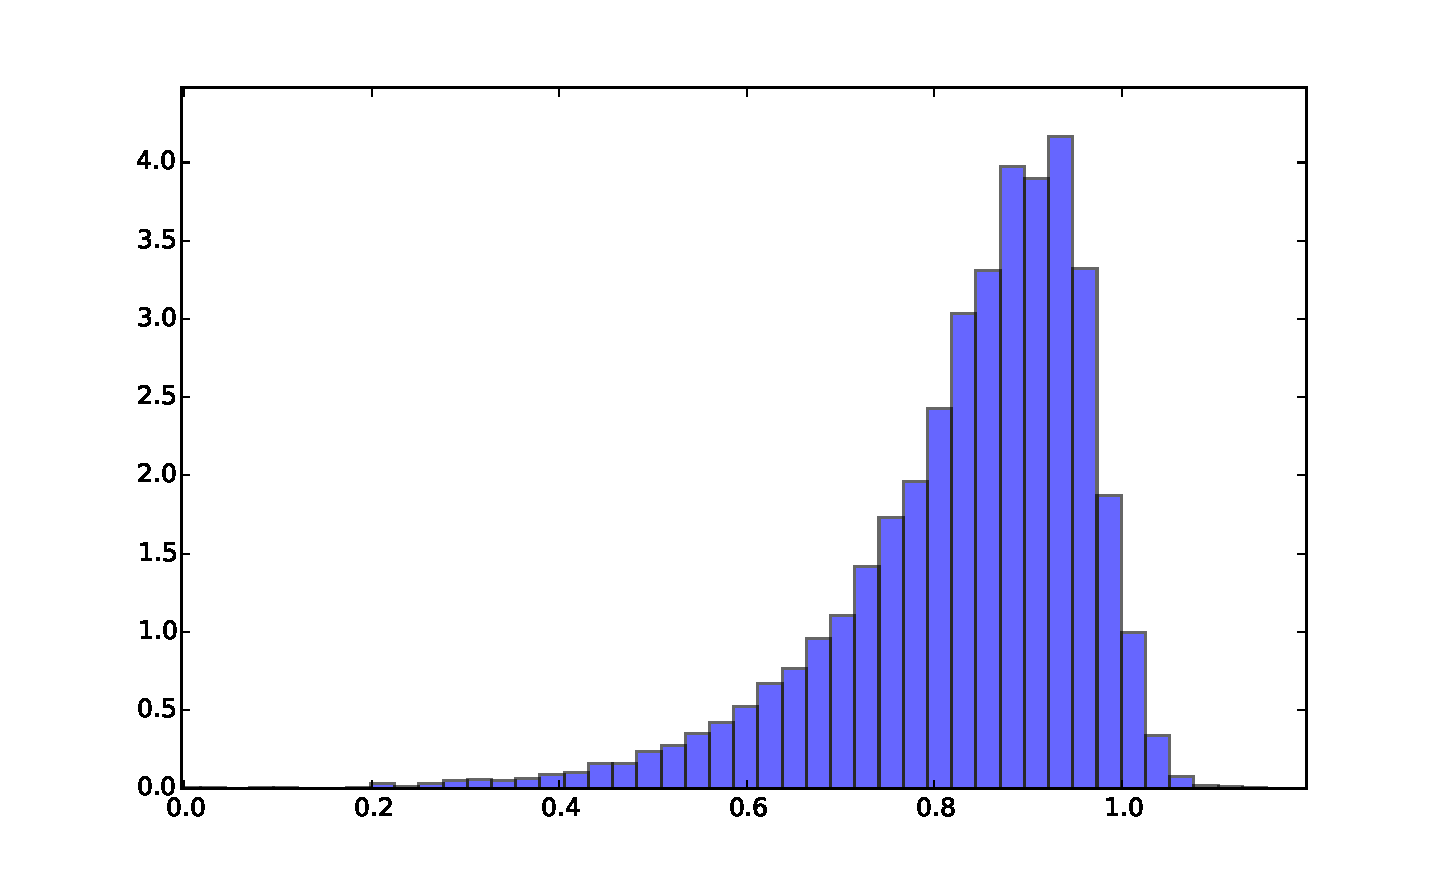
\includegraphics{hghb.pdf}}
        \caption{\label{f:hghb} Observations of $\hat \beta$ when $\beta=0.9$}
       \end{center}
    \end{figure}
    
\end{frame}

\begin{frame}\frametitle{Instrumental Variables}

    \vspace{2em}
    When regressors are endogenous, we can find consistent estimators of $\boldbeta$ when extra information is
    available in the form of ``exogenous" variables called \navy{instruments}
    
    These collected into a $N \times J$ matrix $\boldZ$, where
    each column is observations on one exogenous variable 
    
    \vspace{.7em}
    Assumptions:
    %
    \begin{enumerate}
        \item $\boldy = \boldX \boldbeta + \boldu$
        \item $\EE[ \boldu \given \boldZ] = \boldzero$
        \item $\EE[ \boldu \boldu^\T \given \boldZ] = \sigma^2 \boldI$ for some
            positive constant $\sigma$
        \item $\boldZ^\T \boldX$ has full column rank
    \end{enumerate}


\end{frame}

\begin{frame}
    
    \vspace{2em}
    Assumption 4. implies $J \geq K$
    \begin{itemize}
        \item If $J > K$, the model is said to be \navy{overidentified}
        \item If $J=K$, the model
    is called \navy{exactly identified}
        \item If $J < K$, the model is called
    \navy{underidentified}
    \end{itemize}
    
    \vspace{.7em}
    Multiply $\boldy = \boldX \boldbeta + \boldu$ 
    by $\boldZ^\T$ to produce
    %
    \begin{equation}
        \label{eq:olami}
            \boldZ^\T \boldy = \boldZ^\T \boldX \boldbeta + \boldw
            \quad \text{where} \quad
            \boldw := \boldZ^\T \boldu
    \end{equation}

\end{frame}

\begin{frame}
    
    \vspace{2em}
    Recall the GLS estimator 
    \begin{equation*}
    \hboldbeta_{{\rm GLS}} 
    := (\boldX^\T \boldOmega^{-1} \boldX)^{-1} \boldX^\T \boldOmega^{-1} \boldy
    \end{equation*}

    Substitute $\boldX$ for $\boldZ^\T \boldX$, $\boldy$ for $\boldZ^\T
    \boldy$, and $\boldOmega$ for $\sigma^2 \boldZ^\T \boldZ$
    
    \vspace{.7em}
    The
    \navy{instrumental variable least squares (IVLS) estimator} 
    %
    \begin{equation*}
        \label{eq:ivls}
        \hboldbeta_{{\rm IVLS}} 
        := (\boldX^\T \boldZ (\boldZ^\T \boldZ)^{-1} \boldZ^\T \boldX)^{-1}
        \boldX^\T \boldZ (\boldZ^\T \boldZ)^{-1} \boldZ^\T \boldy
    \end{equation*}
    
    If $J = K$, simplify to 
    %
    \begin{equation*}
        \label{eq:ivls2}
        \hboldbeta_{{\rm IVLS}} 
        := (\boldZ^\T \boldX)^{-1} \boldZ^\T \boldy
    \end{equation*}
        
\end{frame}

\begin{frame}

    \vspace{2em}
    Cannot claim unbiasedness and other properties by
    appealing to the GLS theory --- $\hboldbeta_{{\rm IVLS}}$
    biased in general (see ex.~\ref{ET-ex:ivib})
    \begin{itemize}
        \item because direct
        application of GLS to \eqref{eq:olami} requires  $\EE[ \boldw \given
        \boldZ^\T \boldX] = \boldzero$ rather than $\EE[ \boldw \given \boldZ] =
        \boldzero$
    \end{itemize}
    
    However, bias typically smaller than OLS and vanishes
    asymptotically 
    
    \vspace{.7em}
    Figure:  OLS and IVLS estimates of $\beta$ in
    $y = x \beta + u$ when $\beta=10$:
    
    \begin{itemize}
        \item $z$ drawn independently of $u$
        \item $x=\alpha z + (1 - \alpha) u$
        \item $\alpha$ is constant
    \end{itemize}
    
\end{frame}

\begin{frame}

    \begin{figure}
   \centering
   \scalebox{.44}{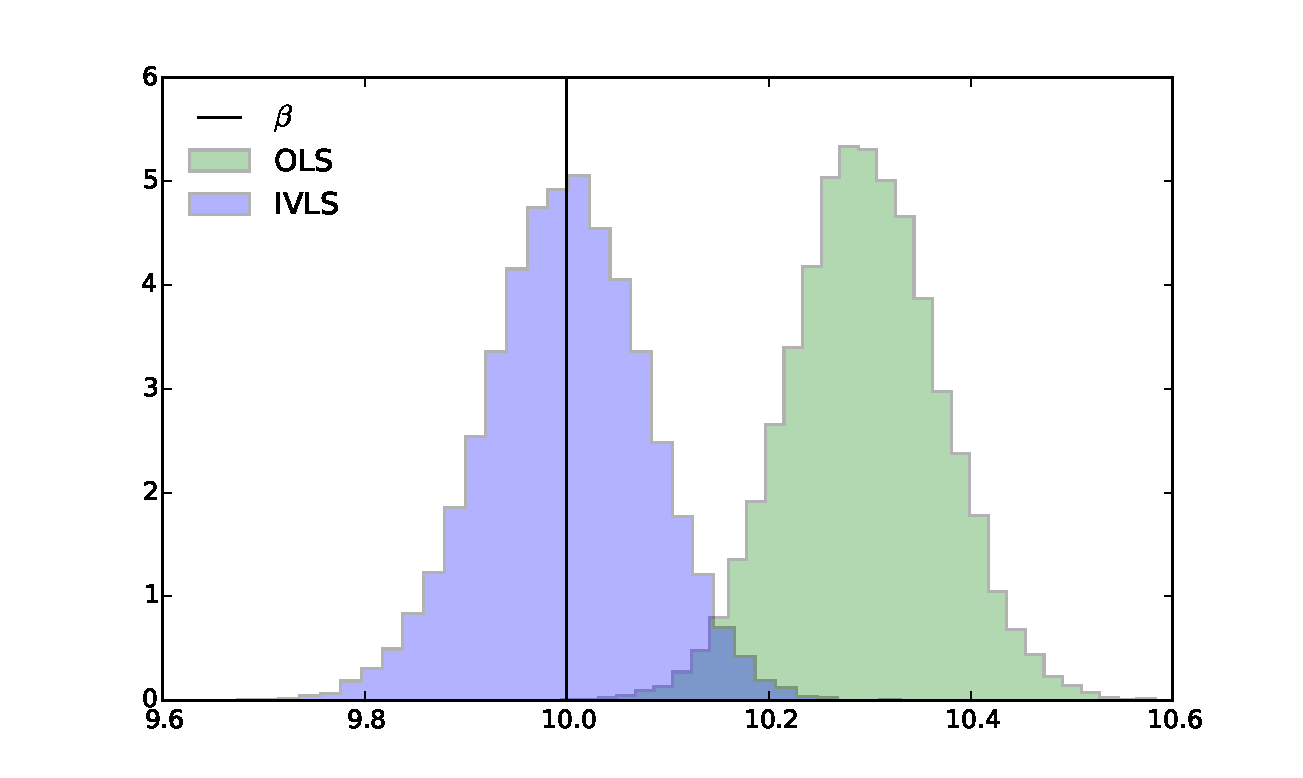
\includegraphics{iv_example.pdf}}
   \caption{\label{f:iv_example} Simulated draws of OLS and IVLS estimators of $\beta$}
    \end{figure}

\end{frame}

\begin{frame}\frametitle{Causality}

    \vspace{2em}
    Interpret $R^2$  as measuring the ``explanatory power''?
    \begin{itemize}
        \item common terminology: ``the total variation in $\boldy$
        is the sum of explained and unexplained variation''
        \item value of $R^2$ claimed to be the fraction of the variation
                in $\boldy$ ``explained'' by the regressors
    \end{itemize}
    
    \vspace{.7em}
    Above terminology misleading: $R^2$ says nothing
    about causation \textit{per se}
    \begin{itemize}
        \item $R^2$ better thought of as a
    measure of correlation 
    \end{itemize}
    
    Understanding causality requires
    either good experiments or good theory --- no magic econometric
    procedure to reliably extract causality from observational


\end{frame}



\end{document}
